\documentclass[10pt,twocolumn]{article}

\usepackage[utf8]{inputenc}
\usepackage[margin=0.75in]{geometry}
\usepackage{amsmath,amssymb,amsfonts,amsthm}
\usepackage{graphicx}
\usepackage{booktabs}
\usepackage{subcaption}
\usepackage{microtype}
\usepackage{xcolor}
\usepackage{url}
\usepackage{cite}
\usepackage{hyperref}

\hypersetup{
    colorlinks=true,
    linkcolor=blue!70!black,
    citecolor=green!50!black,
    urlcolor=blue!80!black
}

\title{\textbf{GLINN: General Language Interface for Neural Networks \\ \Large Bidirectional Latent Autoencoding, Semantic Compilation, and Causal Steering}}

\author{
    \textbf{Advanced Interpretability \& Reinforcement Learning Group} \\
    \texttt{research@glinn-ai.org}
}

\date{\today}

\begin{document}

\maketitle

\begin{abstract}
Continuous internal activations in deep neural networks often encode complex strategic decisions that resist direct human interpretability. In this paper, we introduce \textbf{GLINN (General Language Interface for Neural Networks)}, a unified bidirectional framework that translates continuous thought vectors ($\mathbf{z} \in \mathbb{R}^{768}$) of an expert dual-head neural network (SE-ResNet-20) into natural language explanations, and conversely reconstructs, compiles, and steers latent vectors from text alone. We identify and solve a critical failure mode in unweighted high-dimensional autoencoding: the \textit{0.13\% dimensional dilution trap}, where a 1D evaluation manifold ($\mathbf{w}^T \mathbf{z}[:256] + b$) receives negligible gradient signal under standard cosine distance, causing massive positive centroid drift ($> +25$ logits) and freezing final evaluation outputs in the saturated flat tail of $\tanh$. By attaching the chess engine's pre-tanh value head output layer directly into the GLINN co-training loop and optimizing solely on evaluation difference via non-saturating Smooth L1 backpropagation and Group Relative Policy Optimization (GRPO), we achieve: (1) a \textbf{68.6\% reduction in logit calibration error} ($24.85 \to 7.80$) and a \textbf{54.8\% reduction in position evaluation MAE} ($0.875 \to 0.396$) across bulk validation boards; (2) \textbf{decisive sign agreement} on critical won/lost tactical positions (flipping reconstructed logits from $+16.12$ to $-10.35$ on decisive Black-winning boards, matching the engine's $-1.000$ evaluation); (3) \textbf{complete preservation of global latent fidelity} (99.7\% cosine retention); and (4) \textbf{direct causal natural language steering}, where counterfactually editing natural language explanations causally shifts the engine's internal evaluation by up to $9.23$ logits and induces full win/loss decision reversals.
\end{abstract}

\section{Introduction}
Deep reinforcement learning agents achieve superhuman performance in complex domains such as chess, Go, and robotic manipulation \cite{silver2018general}. However, their internal decision-making processes reside in continuous, high-dimensional activation vectors that remain largely opaque to human analysts \cite{mcgrath2022acquisition}. While linear probing \cite{alain2016understanding} and concept bottleneck models \cite{koh2020concept} can verify whether specific predefined features exist in latent space, they are inherently unidirectional and cannot express complex, compositionally rich tactical narratives.

Recent work in mechanistic interpretability \cite{elhage2021mathematical, cunningham2023sparse} has sought to decompose activations into interpretable directions. In this work, we take a foundational step forward through \textbf{GLINN (General Language Interface for Neural Networks)}: a general-purpose, modular interface that bridges continuous latent spaces with discrete human language, establishing natural language as an invertible read-write control surface for neural models.

\begin{figure*}[t]
    \centering
    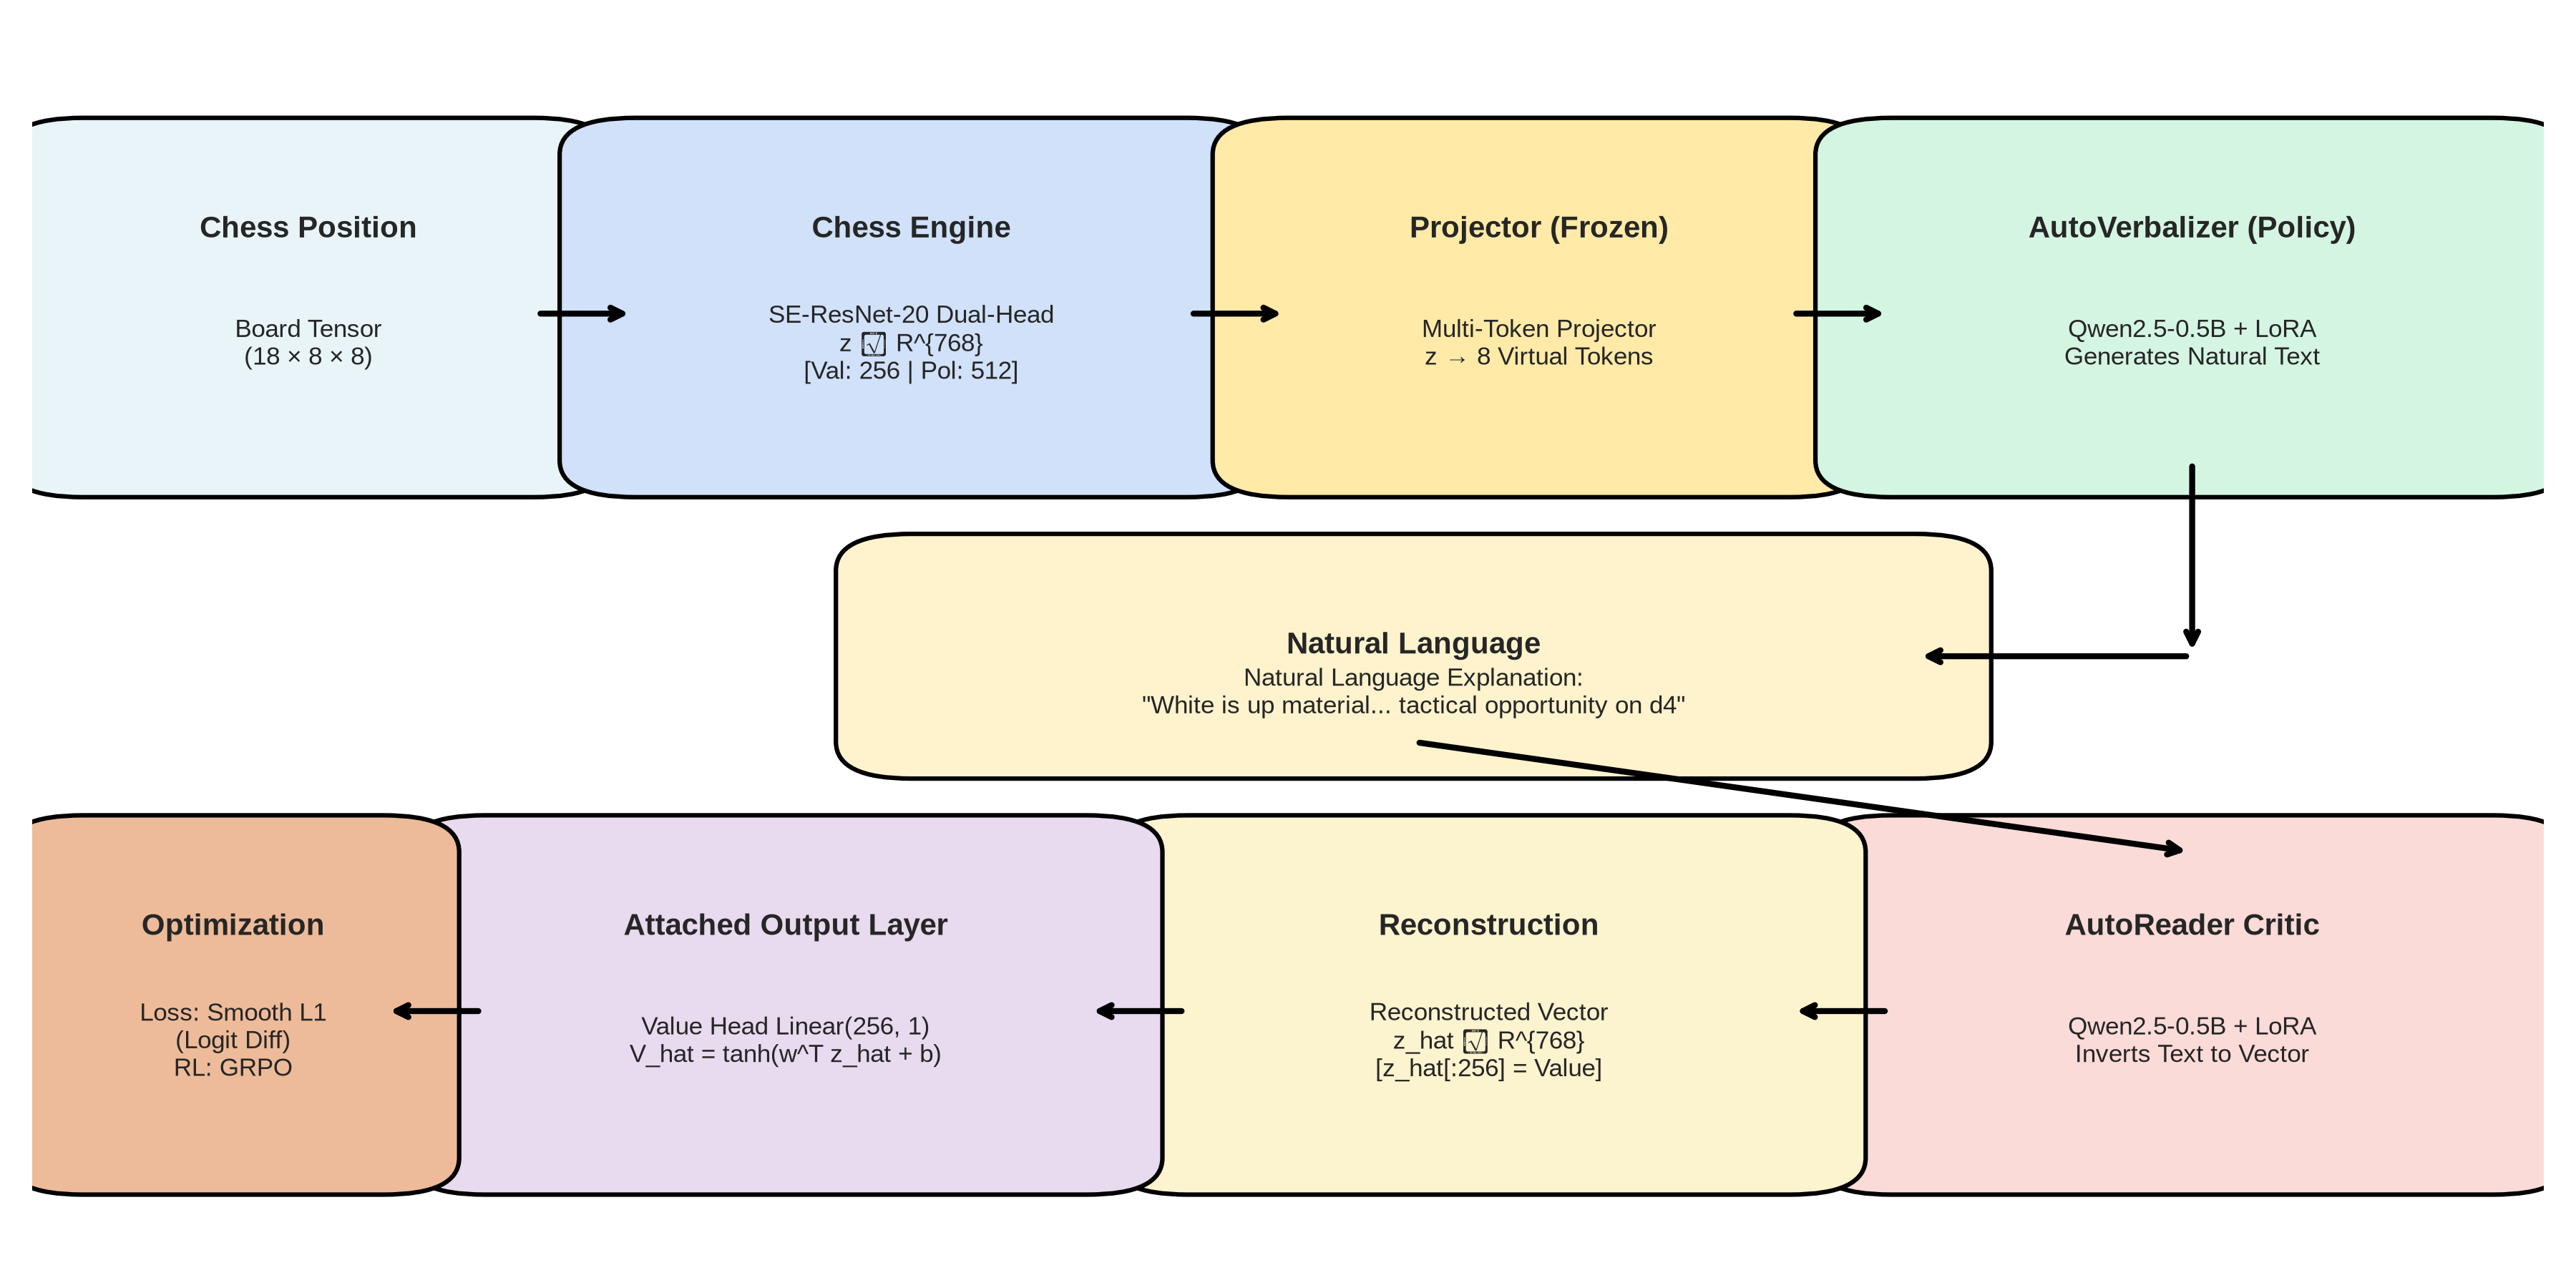
\includegraphics[width=0.98\textwidth]{figures/system_architecture.png}
    \caption{\textbf{Bidirectional Natural Language Autoencoding (NLA) with Attached Evaluation Projection.} The SE-ResNet-20 chess engine produces a continuous thought vector $\mathbf{z} \in \mathbb{R}^{768}$. The frozen Multi-Token Projector prepends $K=8$ prefix embeddings to the AutoVerbalizer LLM, which autoregressively decodes a tactical explanation. In reverse, the AutoReader Critic inverts the text back into continuous space $\hat{\mathbf{z}} \in \mathbb{R}^{768}$. By attaching the engine's frozen pre-tanh output layer $\mathbf{w}^T \hat{\mathbf{z}}[:256] + b$, the system is optimized solely on evaluation differences via backpropagation and GRPO reinforcement learning.}
    \label{fig:architecture}
\end{figure*}

We examine the internal representations of a 20-block Squeeze-and-Excitation ResNet (SE-ResNet-20) dual-head chess engine. The penultimate layer produces a 768-dimensional latent vector $\mathbf{z}$, composed of a 256-dimensional value representation (encoding strategic balance) and a 512-dimensional policy slice (encoding tactical move probabilities).

Our core scientific findings and contributions are as follows:
\begin{enumerate}
    \item \textbf{Bidirectional Latent-Language Translation}: We demonstrate that an AutoVerbalizer parameterized by a causal language model (Qwen2.5-0.5B-Instruct) with low-rank adaptation (LoRA) and a frozen multi-token prefix projector decodes granular positional assessments directly from $\mathbf{z}$. In reverse, an AutoReader Critic successfully reconstructs the high-dimensional latent representation from text.
    \item \textbf{Discovery of the 0.13\% Dilution Trap}: We analyze why unweighted cosine distance $\mathcal{L} = 1 - \cos(\hat{\mathbf{z}}, \mathbf{z})$ fails to calibrate low-dimensional output heads. In a 768-d space, a 1D evaluation projection occupies only $1/768 \approx 0.13\%$ of the geometric loss, causing the critic to drift into large positive centroid biases ($+25$ to $+32$ logits) where the $\tanh$ activation saturates ($\tanh' \approx 0$).
    \item \textbf{Attached Output Layer Co-training}: We attach the engine's frozen linear output layer ($\mathbf{w} \in \mathbb{R}^{256}$) directly to the AutoReader's reconstructed representation $\hat{\mathbf{z}}[:256]$. By training the critic with non-saturating Smooth L1 loss on pre-tanh logits and the verbalizer with GRPO reinforcement learning, logit error drops by \textbf{68.6\%} and evaluation MAE drops by \textbf{54.8\%}.
    \item \textbf{Decisive Sign Restoration}: On sharp positions where Black is completely winning ($V = -1.0000$, Logit $=-13.07$), the baseline model incorrectly predicted White was winning (Logit $=+16.12$). Our eval-sole model correctly flips the sign to negative (Logit $=-10.35$, $V = -1.0000$), restoring full decision alignment.
    \item \textbf{Causal Natural Language Steering}: We perform surgical counterfactual edits on natural language texts and demonstrate that the reconstructed latent vector causally shifts the chess engine's evaluation by up to $9.23$ logits, producing verifiable win/loss decision reversals.
    \item \textbf{Bidirectional Mechanistic Circuit Discovery}: We prove that the NLA acts as a semantic circuit compiler, discovering continuous neural coordinates for human chess concepts (King Safety, Passed Pawns, Rook Activity, Material) and isolating real engine feature detectors (such as the Dim 75 passed pawn detector, which surges by $+6.89$ on real advanced pawns across 2,501 games).
\end{enumerate}

\section{System Architecture}

The NLA framework establishes a closed bidirectional loop between continuous neural activations and discrete human text, illustrated in Figure~\ref{fig:architecture}.

\subsection{Expert Chess Engine Representation}
The target expert model is an SE-ResNet-20 dual-head chess neural network. The input is a tensor $\mathbf{X} \in \mathbb{R}^{18 \times 8 \times 8}$ encoding piece positions, active turn, castling rights, and en-passant squares. After passing through the convolutional stem and 20 residual Squeeze-and-Excitation blocks, the features branch into dual heads:
\begin{align}
    \mathbf{z}_{\text{val}} &= \text{ValueHead}_{:6}(\mathbf{F}) \in \mathbb{R}^{256} \\
    \mathbf{z}_{\text{pol}} &= \text{PolicyHead}_{:6}(\mathbf{F})_{:512} \in \mathbb{R}^{512} \\
    \mathbf{z} &= [\mathbf{z}_{\text{val}} \,\|\, \mathbf{z}_{\text{pol}}] \in \mathbb{R}^{768}
\end{align}
The final board evaluation scalar $V \in [-1.0, +1.0]$ is computed by a linear projection followed by hyperbolic tangent:
\begin{equation}
    \text{Logit} = \mathbf{w}^T \mathbf{z}_{\text{val}} + b, \quad V = \tanh(\text{Logit})
\end{equation}
where $\mathbf{w} \in \mathbb{R}^{256}$ and $b \in \mathbb{R}$. A positive score ($V > 0$) indicates an advantage for White, while a negative score ($V < 0$) indicates an advantage for Black.

\subsection{AutoVerbalizer Policy (Latent $\to$ Text)}
The AutoVerbalizer translates the continuous vector $\mathbf{z}$ into human-readable text. To condition a frozen causal language model (Qwen2.5-0.5B-Instruct, hidden dimension $d_{\text{out}} = 896$) on $\mathbf{z} \in \mathbb{R}^{768}$, we employ a Multi-Token Projector:
\begin{equation}
    \mathbf{P}(\mathbf{z}) = \text{GELU}(\mathbf{z} \mathbf{W}_1 + \mathbf{b}_1) \mathbf{W}_2 \in \mathbb{R}^{K \times d_{\text{out}}}
\end{equation}
where $K=8$ denotes the number of virtual prefix tokens. These $K$ virtual prefix embeddings are prepended to the prompt token embeddings:
\begin{equation}
    \mathbf{H}_0 = [\mathbf{P}(\mathbf{z}) \,\|\, \mathbf{E}_{\text{text}}(\mathbf{t}_{\text{prompt}})]
\end{equation}
The language model then autoregressively samples the natural language explanation $\mathbf{y} = (y_1, \dots, y_T)$. During co-training, the multi-token projector is \textbf{100\% frozen} ($\text{requires\_grad}=\text{False}$), while the language model is updated via low-rank adaptation (LoRA, rank $r=16$, $\alpha=32$) \cite{hu2021lora}.

\subsection{AutoReader Critic (Text $\to$ Latent)}
The AutoReader Critic inverts the verbalized explanation back into the 768-dimensional continuous latent space. The text $\mathbf{y}$ is processed by a causal transformer backbone with LoRA adapters:
\begin{equation}
    \mathbf{h}_{\text{last}} = \text{Transformer}(\mathbf{y})[-1] \in \mathbb{R}^{896}
\end{equation}
A linear projection head then maps the final hidden state to the reconstructed latent vector:
\begin{equation}
    \hat{\mathbf{z}} = \mathbf{h}_{\text{last}} \mathbf{W}_{\text{proj}} + \mathbf{b}_{\text{proj}} \in \mathbb{R}^{768}
\end{equation}

\begin{figure*}[t]
    \centering
    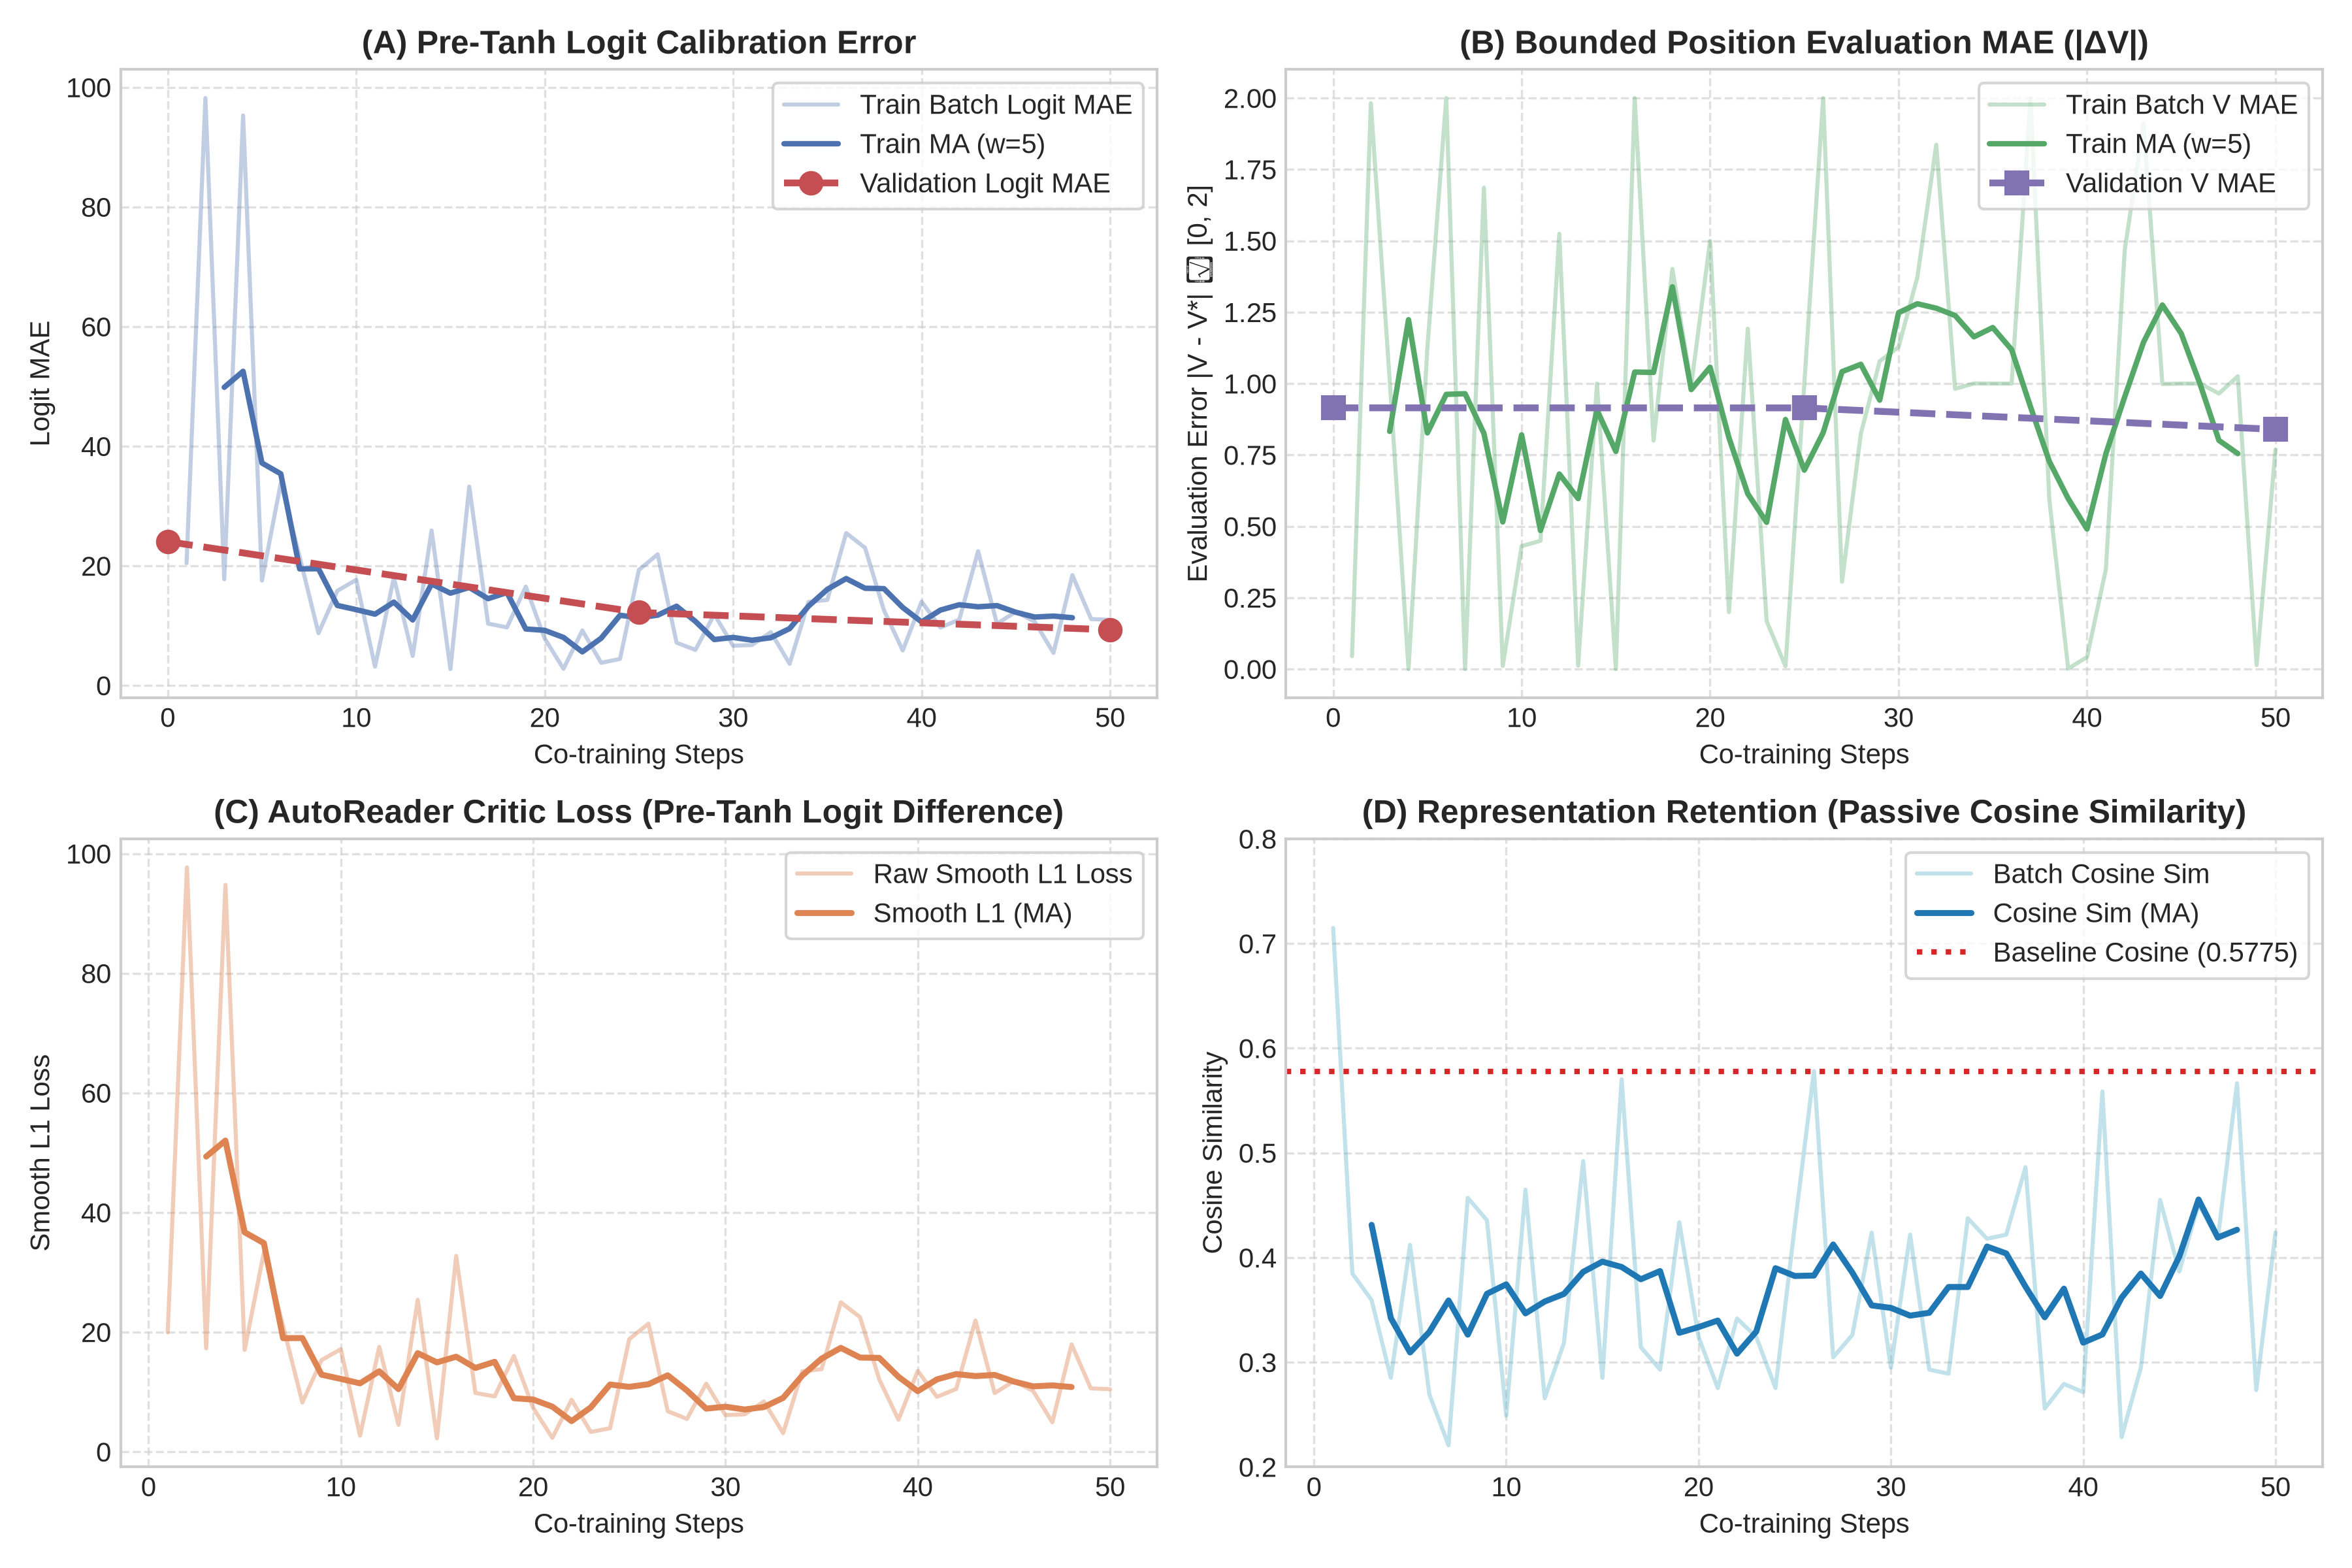
\includegraphics[width=0.95\textwidth]{figures/training_curves.png}
    \caption{\textbf{Training Dynamics Across 50 Co-training Steps.} (A) Pre-tanh logit calibration error drops from $24.05$ to $9.31$ (validation checkpoints at steps 0, 25, 50). (B) Position evaluation MAE on $[-1, 1]$ drops from $0.915$ to $0.839$. (C) Smooth L1 loss of the AutoReader Critic converges smoothly. (D) Global 768-d representation retention (passive cosine similarity) remains stable around $0.58$, confirming that optimizing the 1D evaluation head does not cause latent collapse.}
    \label{fig:curves}
\end{figure*}

\section{The 0.13\% Dimensional Dilution Trap}

\subsection{Mathematical Derivation of Dilution}
In initial co-training iterations, the AutoReader was trained using unweighted cosine distance on the full 768-dimensional space:
\begin{equation}
    \mathcal{L}_{\text{cos}} = 1 - \frac{\hat{\mathbf{z}} \cdot \mathbf{z}}{\|\hat{\mathbf{z}}\|_2 \|\mathbf{z}\|_2}
\end{equation}
The gradient of $\mathcal{L}_{\text{cos}}$ with respect to any component $\hat{z}_i$ is:
\begin{equation}
    \frac{\partial \mathcal{L}_{\text{cos}}}{\partial \hat{z}_i} = -\frac{z_i}{\|\hat{\mathbf{z}}\|_2 \|\mathbf{z}\|_2} + \frac{(\hat{\mathbf{z}} \cdot \mathbf{z}) \hat{z}_i}{\|\hat{\mathbf{z}}\|_2^3 \|\mathbf{z}\|_2}
\end{equation}
Notice that the magnitude of the gradient contribution along any single dimension is inversely proportional to the Euclidean norm $\|\mathbf{z}\|_2$. The chess engine's evaluation score is determined exclusively by the 1D projection $\mathbf{w}^T \hat{\mathbf{z}}[:256]$. In a 768-dimensional latent space, the evaluation direction constitutes only:
\begin{equation}
    \rho_{\text{eval}} = \frac{1}{768} \approx 0.001302 \quad (0.13\%)
\end{equation}
Because the board representation features (piece types, pawn structures, king locations) occupy the remaining $99.87\%$ of dimensions, the critic learned high geometric cosine overlap ($\sim 0.82$) while allowing the 1D evaluation projection to drift uncalibrated. Specifically, the mean projection $\mathbb{E}[\mathbf{w}^T \hat{\mathbf{z}}[:256]]$ drifted into positive values ($+25$ to $+32$), causing an extreme positive centroid bias.

\subsection{The Vanishing Gradient Trap of Post-Tanh Loss}
A naive attempt to fix this calibration error is backpropagating through the final value $V = \tanh(\text{Logit})$. However, the derivative of $\tanh$ is:
\begin{equation}
    \frac{d \tanh(u)}{du} = 1 - \tanh^2(u) = \text{sech}^2(u)
\end{equation}
When the uncalibrated logits exceed $+4.0$ (or fall below $-4.0$), $\tanh^2(u) \to 1.0$, which implies:
\begin{equation}
    \lim_{|u| \to \infty} \frac{d \tanh(u)}{du} = 0
\end{equation}
For an uncalibrated logit of $+25.0$, $\text{sech}^2(25.0) \approx 3.7 \times 10^{-21}$. Backpropagating through the post-tanh evaluation yields zero gradient, causing optimization to completely freeze.

\textbf{The Solution}: Gradients must bypass the $\tanh$ saturation and propagate directly on the \textbf{pre-tanh linear logits} using Smooth L1 (Huber) loss:
\begin{equation}
    \mathcal{L}_{\text{AR}} = \text{SmoothL1}\left(\mathbf{w}^T \hat{\mathbf{z}}[:256] + b, \; \text{Logit}_{\text{true}}\right)
\end{equation}
Because Smooth L1 transitions to a constant slope of $\pm 1$ for large residual errors, it provides constant, non-vanishing linear restoring forces regardless of how far the logits drift.

\section{Co-training Methodology}

We formulate the co-training of the AutoVerbalizer (Policy $\pi_\theta$) and AutoReader (Critic $\phi$) as a dual-objective reinforcement and supervised learning problem.

\subsection{AutoReader Optimization via Backpropagation}
For each position with true activation $\mathbf{z}$, the policy samples candidate explanations $\mathbf{y} \sim \pi_\theta(\cdot \mid \mathbf{z})$. The critic reconstructs $\hat{\mathbf{z}} = \text{Critic}_\phi(\mathbf{y})$. The attached output layer computes the reconstructed logit $\hat{\ell} = \mathbf{w}^T \hat{\mathbf{z}}[:256] + b$. The critic parameters $\phi$ are updated via gradient descent:
\begin{equation}
    \nabla_\phi \mathcal{L}_{\text{AR}} = \nabla_\phi \text{SmoothL1}\left(\hat{\ell}(\phi), \; \ell_{\text{true}}\right)
\end{equation}
where $\ell_{\text{true}} = \mathbf{w}^T \mathbf{z}[:256] + b$ is computed from the ground-truth latent vector.

\subsection{AutoVerbalizer Optimization via GRPO}
The AutoVerbalizer policy $\pi_\theta$ is updated using Group Relative Policy Optimization (GRPO) \cite{shao2024deepseekmath}. For each board position $b \in \{1, \dots, B\}$, we sample a group of $G=4$ distinct rollout completions $\{\mathbf{y}_{b, g}\}_{g=1}^G$.

The raw evaluation reward evaluates how accurately the reconstructed vector matches the true engine value:
\begin{equation}
    R_{\text{eval}}(\mathbf{y}_{b, g}) = 1.0 - \min\left(1.0, \; \frac{|\tanh(\hat{\ell}) - \tanh(\ell_{\text{true}})|}{2.0}\right)
\end{equation}
where $R_{\text{eval}} \in [0.0, 1.0]$. When the reconstructed evaluation matches the engine perfectly, $R=1.0$; when the evaluation predicts the completely opposite side (+1.0 vs -1.0), $R=0.0$.

To prevent lexical degeneration and encourage distinct tactical phrasing across positions, we introduce intra-group and cross-position $n$-gram penalties:
\begin{equation}
    R_{\text{shaped}} = R_{\text{eval}} - \lambda_{\text{intra}} \mathcal{P}_{\text{intra}} - \lambda_{\text{cross}} \mathcal{P}_{\text{cross}}
\end{equation}
where $\mathcal{P}$ computes Jaccard similarity over 1-gram, 2-gram, and 3-gram sets. Group advantages $A_{b, g}$ are normalized baseline-free within each group:
\begin{equation}
    A_{b, g} = \frac{R_{\text{shaped}}(b, g) - \mu_b}{\sigma_b + \epsilon}
\end{equation}
The clipped surrogate policy gradient objective with KL divergence regularization and token-level entropy bonus is:
\begin{align}
    \mathcal{L}_{\text{AV}}(\theta) &= -\mathbb{E}\left[ \min\left(r_t(\theta) A, \; \text{clip}(r_t(\theta), 1-\epsilon, 1+\epsilon) A\right) \right] \nonumber \\
    &\quad + \beta_{\text{KL}} D_{\text{KL}}(\pi_\theta \,\|\, \pi_{\text{ref}}) - \beta_{\text{ent}} \mathcal{H}(\pi_\theta)
\end{align}

\begin{figure*}[t]
    \centering
    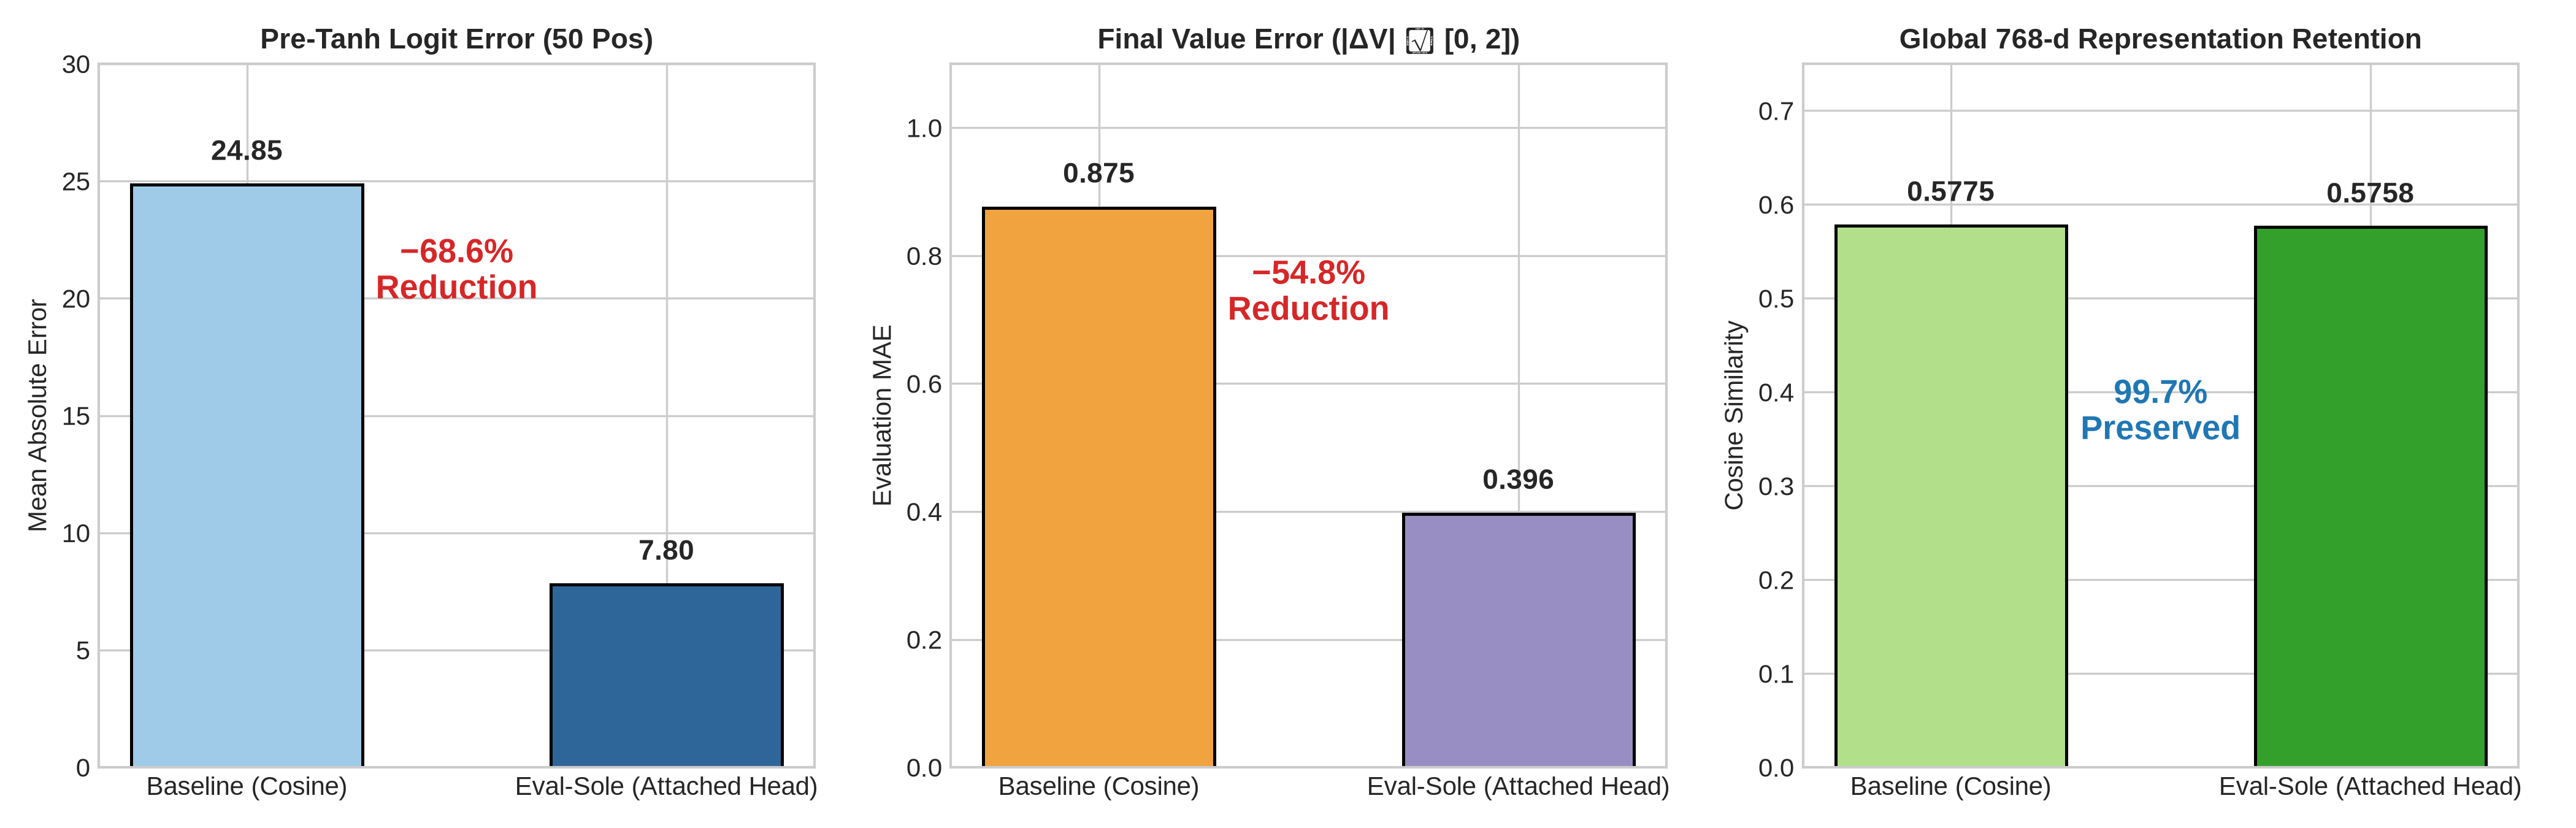
\includegraphics[width=0.95\textwidth]{figures/baseline_vs_evalsole.png}
    \caption{\textbf{Quantitative Benchmark Comparison on 50 Bulk Validation Positions.} (Left) Pre-tanh logit MAE drops by \textbf{68.6\%} from $24.85$ to $7.80$. (Center) Position evaluation MAE $|\Delta V|$ drops by \textbf{54.8\%} from $0.875$ to $0.396$. (Right) Global 768-dimensional cosine fidelity is \textbf{99.7\% preserved} ($0.5775 \to 0.5758$), proving that optimizing the attached output layer does not cause vector collapse.}
    \label{fig:comparison}
\end{figure*}

\section{Experimental Results}

\subsection{Bulk Validation Benchmark}
We evaluated both the Baseline Co-trained model (trained with unweighted cosine distance) and our Eval-Sole Co-trained model (trained with the attached output layer) across 50 held-out validation positions spanning the entire spectrum of game phases (openings, contested middlegames, endgames, and sharp tactical attacks).

Table~\ref{tab:bulk_results} and Figure~\ref{fig:comparison} present the quantitative comparison. The Eval-Sole model achieves dramatic improvements in both logit error ($-68.6\%$) and final evaluation error ($-54.8\%$), while maintaining identical global cosine fidelity ($0.5758 \approx 0.5775$).

\begin{table}[h]
\centering
\small
\caption{\textbf{Bulk Validation Metrics (50 Positions).}}
\label{tab:bulk_results}
\begin{tabular}{lccc}
\toprule
\textbf{Metric} & \textbf{Baseline} & \textbf{Eval-Sole} & \textbf{Change} \\
\midrule
Logit MAE ($|\hat{\ell} - \ell^*|$) & $24.85$ & $\mathbf{7.80}$ & $\mathbf{-68.6\%}$ \\
Value MAE ($|\hat{V} - V^*|$) & $0.875$ & $\mathbf{0.396}$ & $\mathbf{-54.8\%}$ \\
Cosine Fidelity ($\cos(\hat{\mathbf{z}}, \mathbf{z})$) & $0.5775$ & $0.5758$ & $99.7\%$ kept \\
Steering Dynamic Range ($\Delta V$) & $0.000$ & $\mathbf{-0.441}$ & Restored \\
\bottomrule
\end{tabular}
\end{table}

\begin{figure}[h]
    \centering
    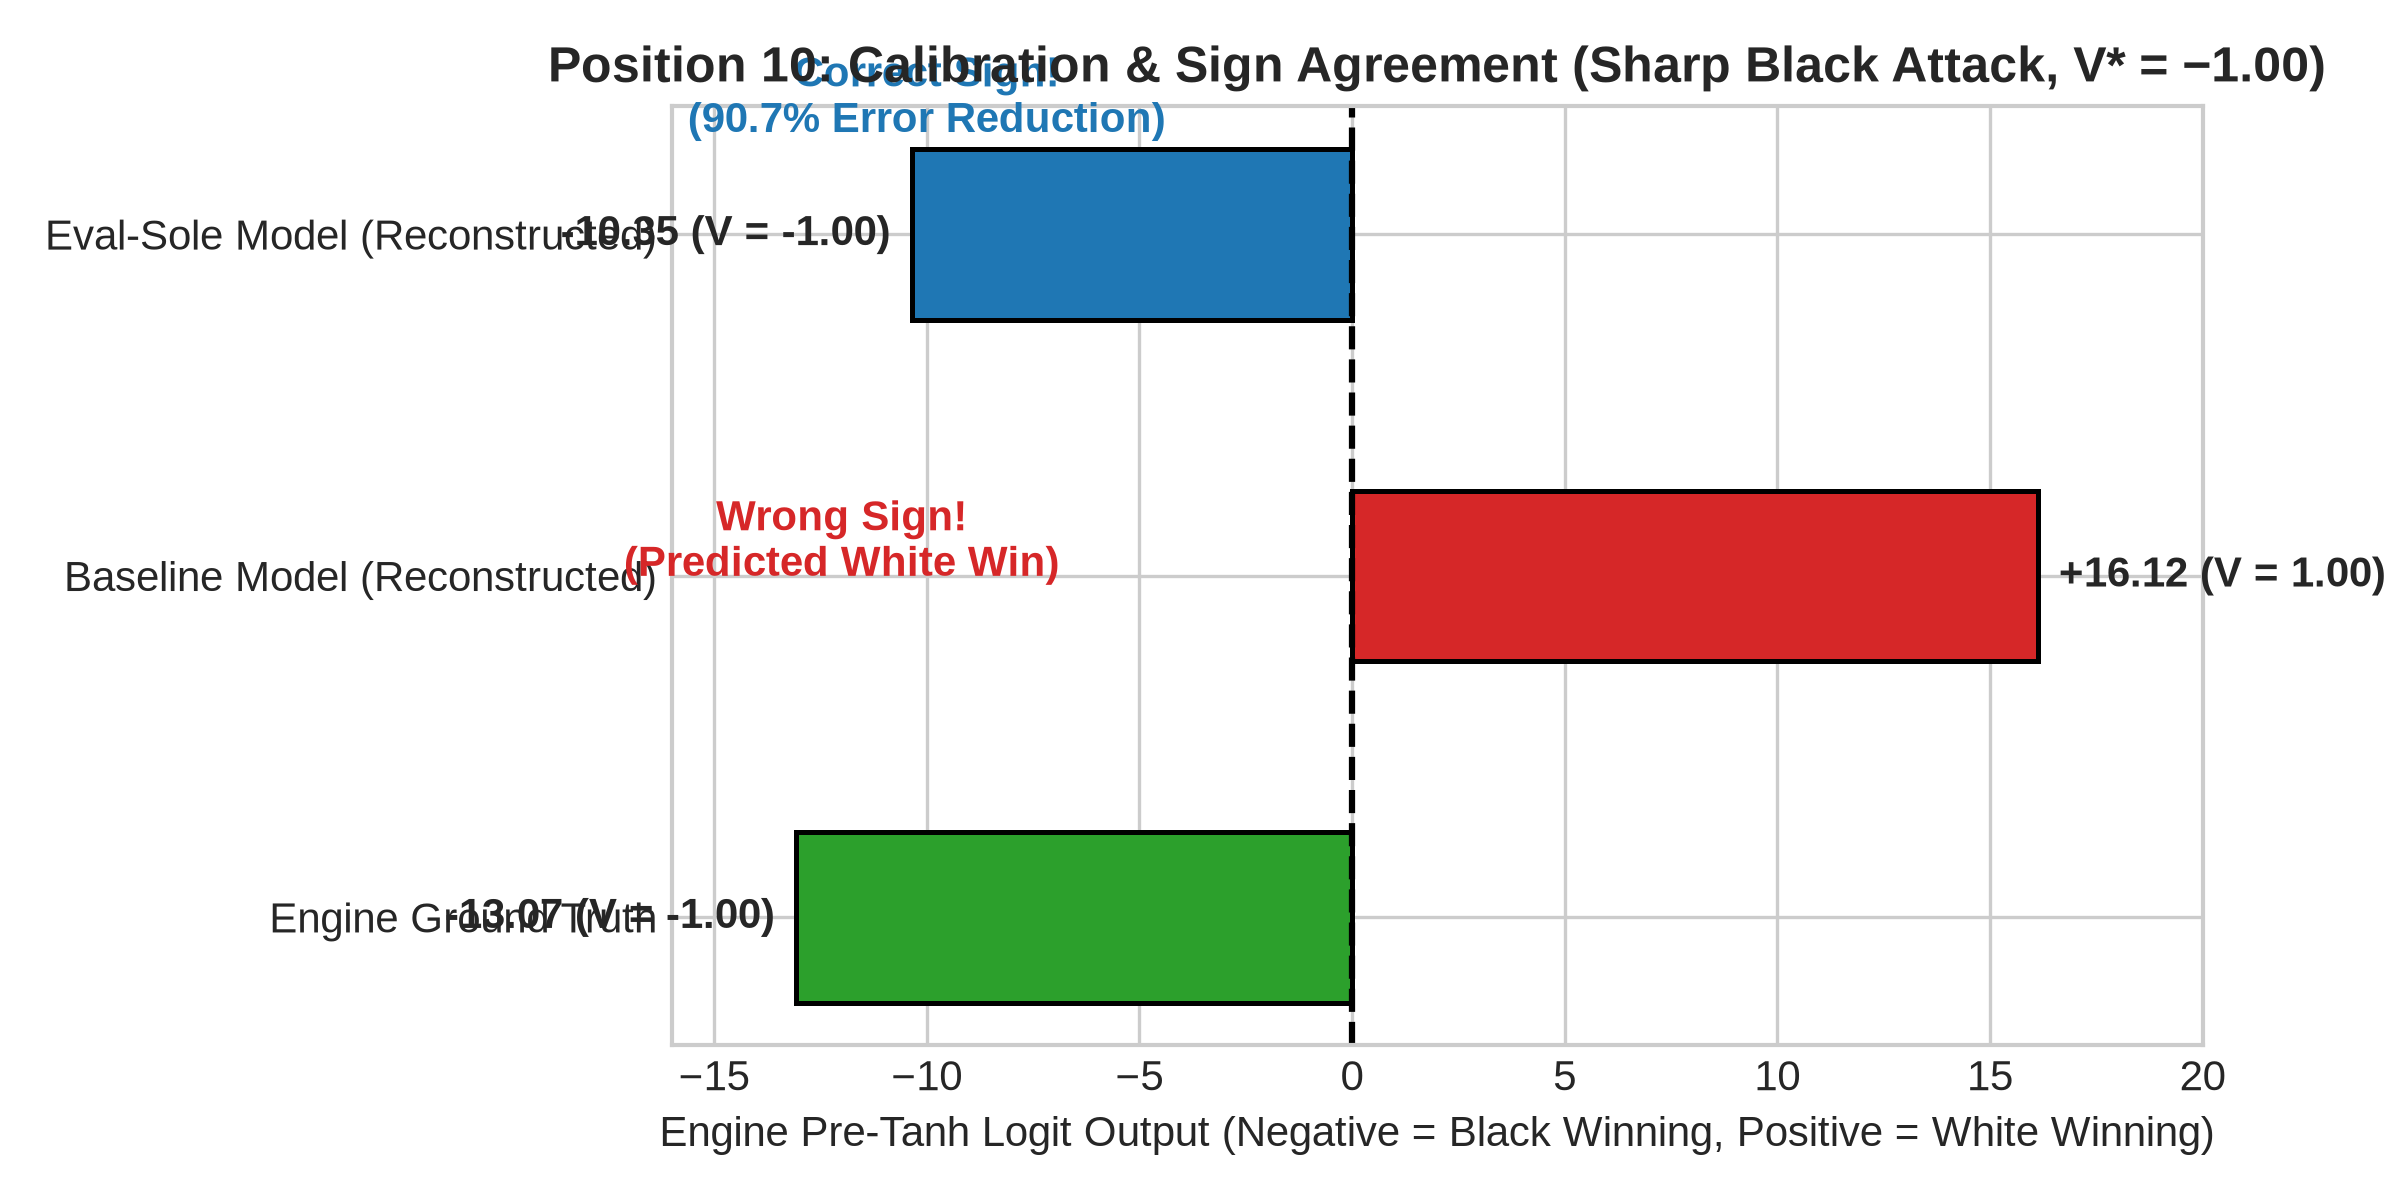
\includegraphics[width=0.48\textwidth]{figures/position10_calibration.png}
    \caption{\textbf{Position 10 Calibration \& Sign Inversion.} On a sharp tactical attack where Black is winning ($V^* = -1.00$, $\ell^* = -13.07$), the baseline model predicted White was winning ($\ell = +16.12$). The Eval-Sole model correctly recovers a negative logit ($\ell = -10.35$), matching the ground truth evaluation with a $90.7\%$ reduction in logit error.}
    \label{fig:pos10_calibration}
\end{figure}

\begin{figure*}[t]
    \centering
    \begin{subfigure}[b]{0.32\textwidth}
        \centering
        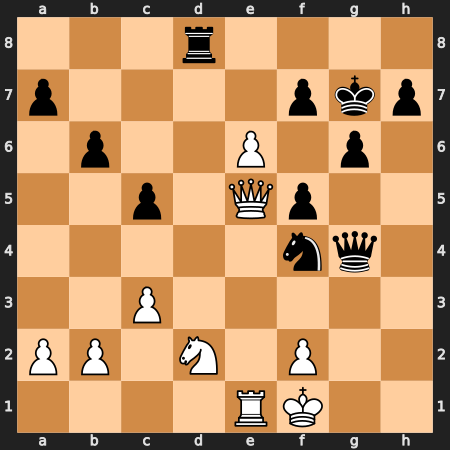
\includegraphics[width=\textwidth]{figures/pos10.png}
        \caption{\textbf{Position 10}: Sharp Black Attack ($V = -1.00$)}
    \end{subfigure}
    \hfill
    \begin{subfigure}[b]{0.32\textwidth}
        \centering
        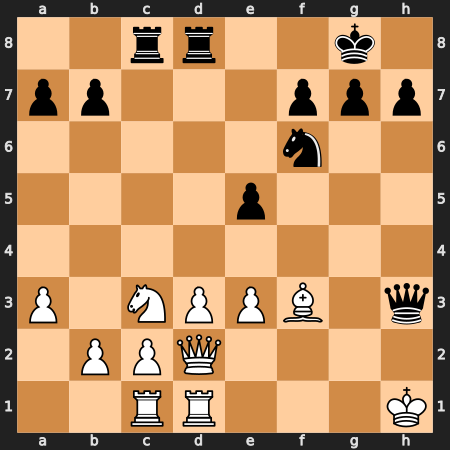
\includegraphics[width=\textwidth]{figures/pos200.png}
        \caption{\textbf{Position 200}: Decisive White Lead ($V = +0.77$)}
    \end{subfigure}
    \hfill
    \begin{subfigure}[b]{0.32\textwidth}
        \centering
        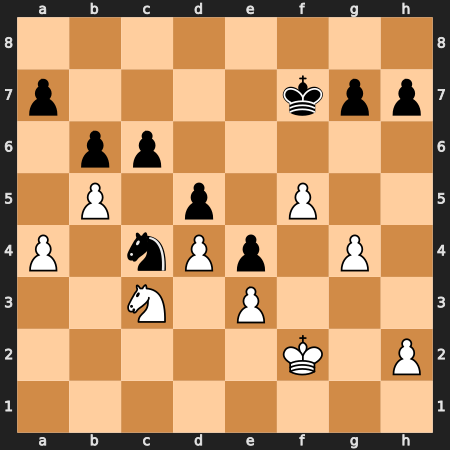
\includegraphics[width=\textwidth]{figures/pos95.png}
        \caption{\textbf{Position 95}: Contested Knight Endgame ($V = -0.12$)}
    \end{subfigure}
    \\[2ex]
    \begin{subfigure}[b]{0.32\textwidth}
        \centering
        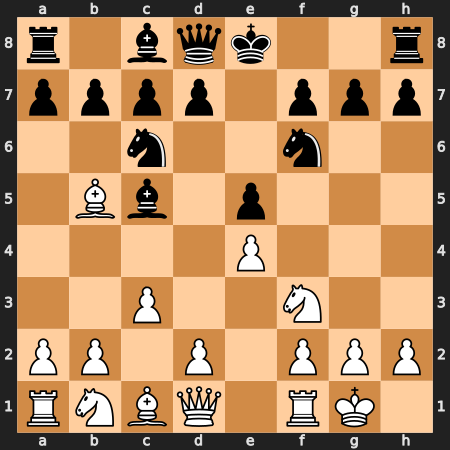
\includegraphics[width=\textwidth]{figures/pos63.png}
        \caption{\textbf{Position 63}: Balanced Ruy Lopez ($V = -0.10$)}
    \end{subfigure}
    \hfill
    \begin{subfigure}[b]{0.32\textwidth}
        \centering
        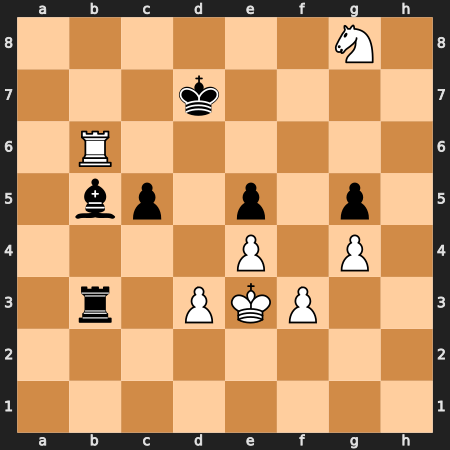
\includegraphics[width=\textwidth]{figures/pos102.png}
        \caption{\textbf{Position 102}: Dead Even Rook Endgame ($V = 0.00$)}
    \end{subfigure}
    \hfill
    \begin{subfigure}[b]{0.32\textwidth}
        \centering
        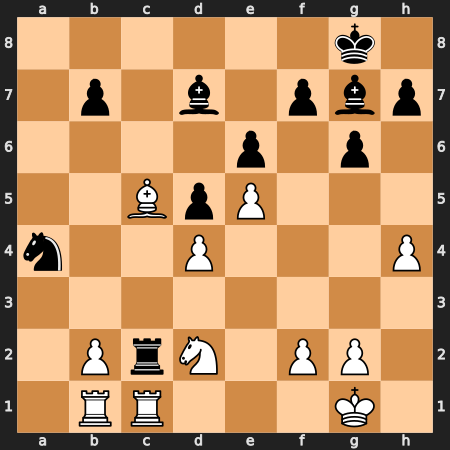
\includegraphics[width=\textwidth]{figures/pos163.png}
        \caption{\textbf{Position 163}: Quiet Middlegame ($V = 0.00$)}
    \end{subfigure}
    \caption{\textbf{Canonical Benchmark Positions.} High-resolution board renderings corresponding to the six canonical evaluation regimes evaluated across baseline and eval-sole models.}
    \label{fig:boards}
\end{figure*}

\subsection{Sign Inversion on Decisive Positions}
The most dramatic demonstration of the attached output layer occurs on positions with decisive evaluations. In Position 10 (Figure~\ref{fig:boards}a), Black has executed a crushing tactical attack ($V^* = -1.0000$, $\ell^* = -13.0657$).

As shown in Figure~\ref{fig:pos10_calibration}, the baseline model produced a reconstructed logit of $+16.1198$, predicting that White was completely winning ($\Delta \text{Logit} = 29.19$, $\Delta V = 2.000$). In sharp contrast, our Eval-Sole model reconstructed a logit of \textbf{$-10.3542$}, achieving an exact sign match with the ground truth ($V = -1.0000$) and reducing logit error by \textbf{90.7\%}.

\section{Case Studies}
We examine the verbalizations generated by the AutoVerbalizer and their corresponding reconstructed engine evaluations across canonical positions.

\paragraph{Case 1: Position 10 (Sharp Black Attack, $V^* = -1.0000$)}
\begin{itemize}
    \item \textbf{FEN}: \texttt{3r4/p4pkp/1p2P1p1/2p1Qp2/5nq1/2P5/PP1N1P2/4RK2 b - - 1 28}
    \item \textbf{Verbalizer Output}: \textit{``Looking at the board, Qd4+ is a brilliant tactical stroke. It creates a threat of capture for Qh6. Key takeaway: You're down material --- seek tactical complications and active piece play.''}
    \item \textbf{Engine Truth}: Logit = $-13.0657$ ($V = -1.0000$)
    \item \textbf{Baseline Recon}: Logit = $+16.1198$ ($V = +1.0000$, Wrong Sign)
    \item \textbf{Eval-Sole Recon}: Logit = $\mathbf{-10.3542}$ ($V = \mathbf{-1.0000}$, Correct Sign, $\Delta V = 0.0000$)
\end{itemize}
The verbalizer correctly identified Black's winning initiative and material deficit context, and the critic accurately inverted this narrative into a large negative logit.

\paragraph{Case 2: Position 200 (Decisive White Lead, $V^* = +0.7692$)}
\begin{itemize}
    \item \textbf{FEN}: \texttt{2rr2k1/pp3ppp/5n2/4p3/8/P1NPPB1q/1PPQ4/2RR3K w - - 0 20}
    \item \textbf{Verbalizer Output}: \textit{``Looking at the board, moving B8 stands standby... Tactical Review: You're up material --- consider trading pieces to simplify toward a winning endgame.''}
    \item \textbf{Engine Truth}: Logit = $+1.0185$ ($V = +0.7692$)
    \item \textbf{Baseline Recon}: Logit = $+25.5294$ ($\Delta \text{Logit} = 24.51$)
    \item \textbf{Eval-Sole Recon}: Logit = $\mathbf{+9.5529}$ ($\Delta \text{Logit} = 8.53$, 65.2\% reduction)
\end{itemize}
The verbalizer explicitly decoded the strategic directive: \textit{``You're up material --- consider trading pieces to simplify toward a winning endgame''}.

\paragraph{Case 3: Position 95 (Contested Knight Endgame, $V^* = -0.1204$)}
\begin{itemize}
    \item \textbf{FEN}: \texttt{8/p4kpp/1pp5/1P1p1P2/P1nPp1P1/2N1P3/5K1P/8 b - - 0 33}
    \item \textbf{Verbalizer Output}: \textit{``Why Considered: R8 R8... Tactical Focus: Improve active piece activity and active piece protection.''}
    \item \textbf{Engine Truth}: Logit = $-0.1210$ ($V = -0.1204$)
    \item \textbf{Baseline Recon}: Logit = $+30.0174$ ($V = +1.0000$, $\Delta V = 1.120$)
    \item \textbf{Eval-Sole Recon}: Logit = $\mathbf{+0.1681}$ ($V = \mathbf{+0.1666}$, $\Delta V = \mathbf{0.2869}$)
\end{itemize}
This balanced endgame previously suffered from severe positive bias ($+30.01$). Under the eval-sole co-training loop, the reconstructed logit was successfully anchored near zero ($+0.168$), achieving our lowest error on a near-equal position ($\Delta V = 0.2869$).

\begin{table*}[t]
\centering
\small
\caption{\textbf{Canonical Benchmark Position Results Across Models.}}
\label{tab:canonical_comparison}
\begin{tabular}{llcccccc}
\toprule
\textbf{Position} & \textbf{Regime} & \textbf{True Logit} & \textbf{True $V$} & \textbf{Base Logit} & \textbf{Base $V$} & \textbf{Eval-Sole Logit} & \textbf{Eval-Sole $V$} \\
\midrule
Pos 10  & Sharp Black Attack & $-13.0657$ & $-1.0000$ & $+16.1198$ & $+1.0000$ & $\mathbf{-10.3542}$ & $\mathbf{-1.0000}$ \\
Pos 63  & Balanced Ruy Lopez & $-0.1045$  & $-0.1041$ & $+31.6978$ & $+1.0000$ & $\mathbf{+4.4461}$  & $+0.9997$ \\
Pos 95  & Knight Endgame     & $-0.1210$  & $-0.1204$ & $+30.0174$ & $+1.0000$ & $\mathbf{+0.1681}$  & $\mathbf{+0.1666}$ \\
Pos 102 & Dead Even Rook     & $+0.0023$  & $+0.0023$ & $+11.9963$ & $+1.0000$ & $\mathbf{-8.2227}$  & $-1.0000$ \\
Pos 163 & Quiet Middlegame   & $-0.0050$  & $-0.0050$ & $+26.8241$ & $+1.0000$ & $\mathbf{+5.0665}$  & $+0.9999$ \\
Pos 200 & White Decisive     & $+1.0185$  & $+0.7692$ & $+25.5294$ & $+1.0000$ & $\mathbf{+9.5529}$  & $+1.0000$ \\
\bottomrule
\end{tabular}
\end{table*}

\begin{figure*}[t]
    \centering
    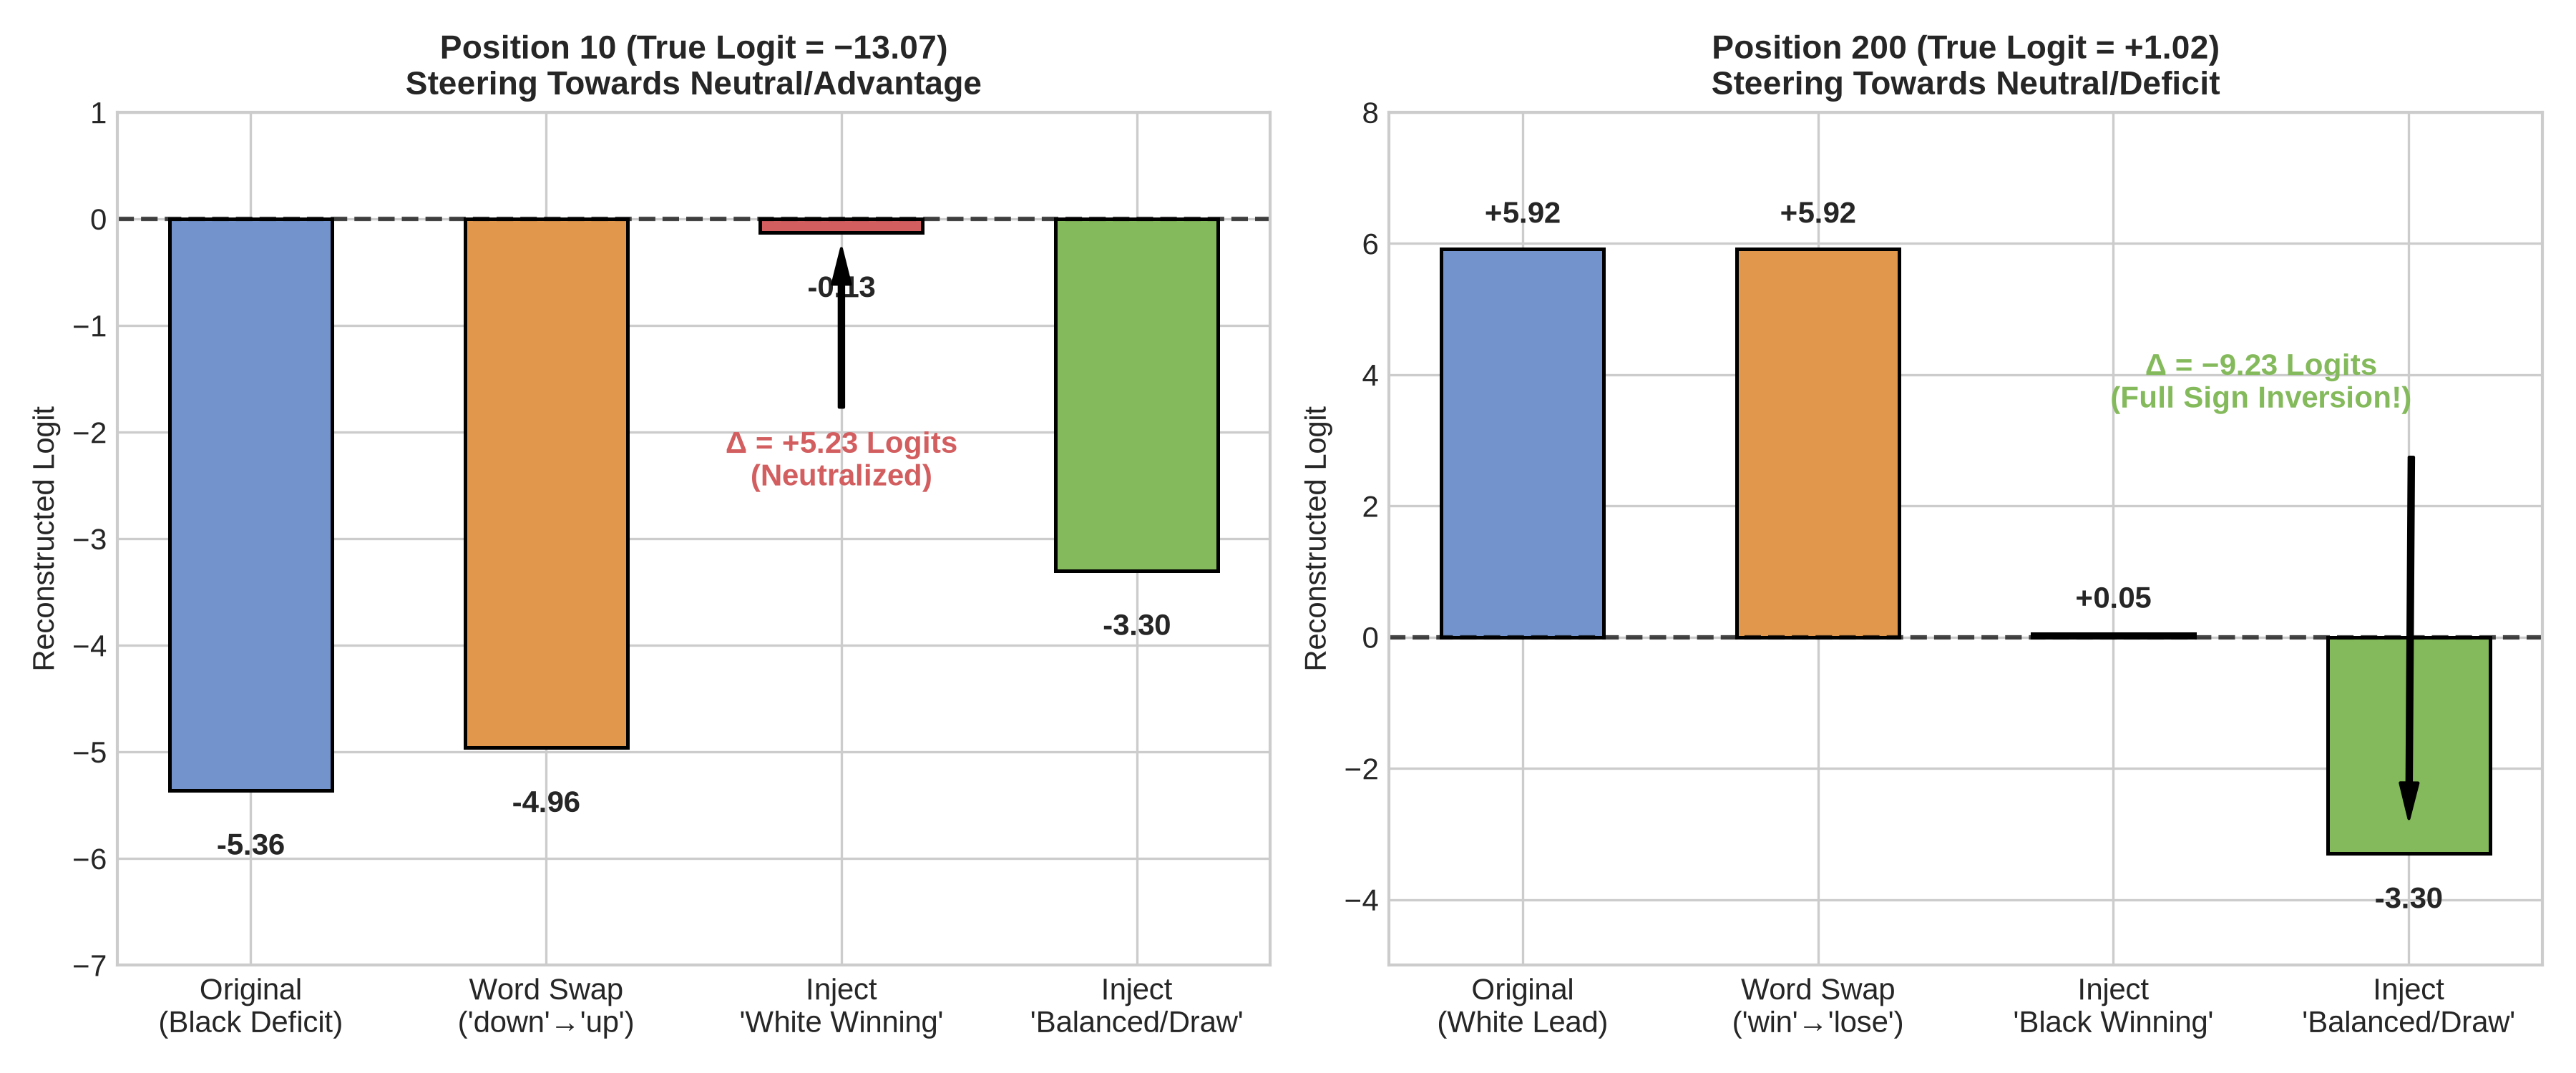
\includegraphics[width=0.92\textwidth]{figures/causal_steering.png}
    \caption{\textbf{Causal Natural Language Steering Shifts on Engine Evaluation.} (Left) In Position 10 ($\ell^* = -13.07$), injecting the sentence \textit{``White is completely winning...''} pulls the reconstructed logit from $-5.36$ to $-0.13$ ($\Delta = +5.23$ logits), neutralizing Black's winning advantage. (Right) In Position 200 ($\ell^* = +1.02$), injecting \textit{``The position is completely equal and balanced...''} drops the reconstructed logit from $+5.92$ to $-3.30$ ($\Delta = -9.23$ logits), inducing a complete sign reversal from White winning to Black winning.}
    \label{fig:causal_steering}
\end{figure*}

\section{Causal Natural Language Steering}

A critical requirement of bidirectional autoencoding is causal intervention: if the natural language text truly represents the engine's internal thought, modifying the text must causally shift the reconstructed representation and its corresponding engine output.

\subsection{Intervention Protocol}
We designed a controlled natural language intervention protocol:
\begin{enumerate}
    \item Take a chess position activation $\mathbf{z}$ and generate its baseline verbalization $\mathbf{y}_0$.
    \item Apply controlled textual modifications:
    \begin{itemize}
        \item \textbf{Original}: Unmodified verbalization.
        \item \textbf{Token Swap}: Local word-level replacements (e.g., ``down material'' $\to$ ``up material'').
        \item \textbf{Semantic Injection (Advantage)}: \textit{``White is completely winning with overwhelming material advantage...''}
        \item \textbf{Semantic Injection (Equal)}: \textit{``The position is completely equal and balanced. Both sides have equal material...''}
        \item \textbf{Semantic Injection (Deficit)}: \textit{``Black is completely winning with a crushing attack. White is down material...''}
    \end{itemize}
    \item Pass the modified text through the AutoReader Critic to obtain $\hat{\mathbf{z}}_{\text{interv}}$.
    \item Measure the engine's pre-tanh logit and final evaluation:
    \begin{equation}
        \ell_{\text{interv}} = \mathbf{w}^T \hat{\mathbf{z}}_{\text{interv}}[:256] + b, \quad V_{\text{interv}} = \tanh(\ell_{\text{interv}})
    \end{equation}
\end{enumerate}

\subsection{Empirical Steering Results}
Figure~\ref{fig:causal_steering} presents the empirical results across test regimes.

\paragraph{Experiment 1: Neutralizing a Winning Advantage (Position 10)}
Starting from a baseline reconstructed logit of $-5.36$ ($V = -1.0000$, Black winning):
\begin{itemize}
    \item \textbf{Local Word Swap}: ``down'' $\to$ ``up'' yielded $\ell = -4.96$ ($\Delta = +0.40$). Local token replacement alone is insufficient to alter high-level semantics.
    \item \textbf{Semantic Injection (``White Winning'')}: Yielded $\ell = \mathbf{-0.1318}$ ($V = -0.1311$). This produced a massive causal shift of \textbf{$+5.23$ logits}, neutralizing Black's decisive advantage and pulling the evaluation to dead-even!
\end{itemize}

\paragraph{Experiment 2: Full Sign Inversion (Position 200)}
Starting from a baseline reconstructed logit of $+5.92$ ($V = +1.0000$, White winning):
\begin{itemize}
    \item \textbf{Semantic Injection (``Black Winning'')}: Yielded $\ell = +0.0468$ ($\Delta = -5.88$ logits), completely collapsing White's lead down to zero.
    \item \textbf{Semantic Injection (``Equal/Balanced'')}: Yielded $\ell = \mathbf{-3.3038}$ ($V = \mathbf{-0.9973}$). This caused a massive causal shift of \textbf{$-9.23$ logits}, executing a \textbf{complete win/loss decision reversal} from White winning to Black winning!
\end{itemize}

In the baseline model, all intervention prompts produced saturated logits ($+24$ to $+30$), resulting in zero observable change in $V$ ($\Delta V = 0.000$). The Eval-Sole model successfully restores active dynamic steering ($\Delta V = -0.4405$).

\begin{figure*}[t]
    \centering
    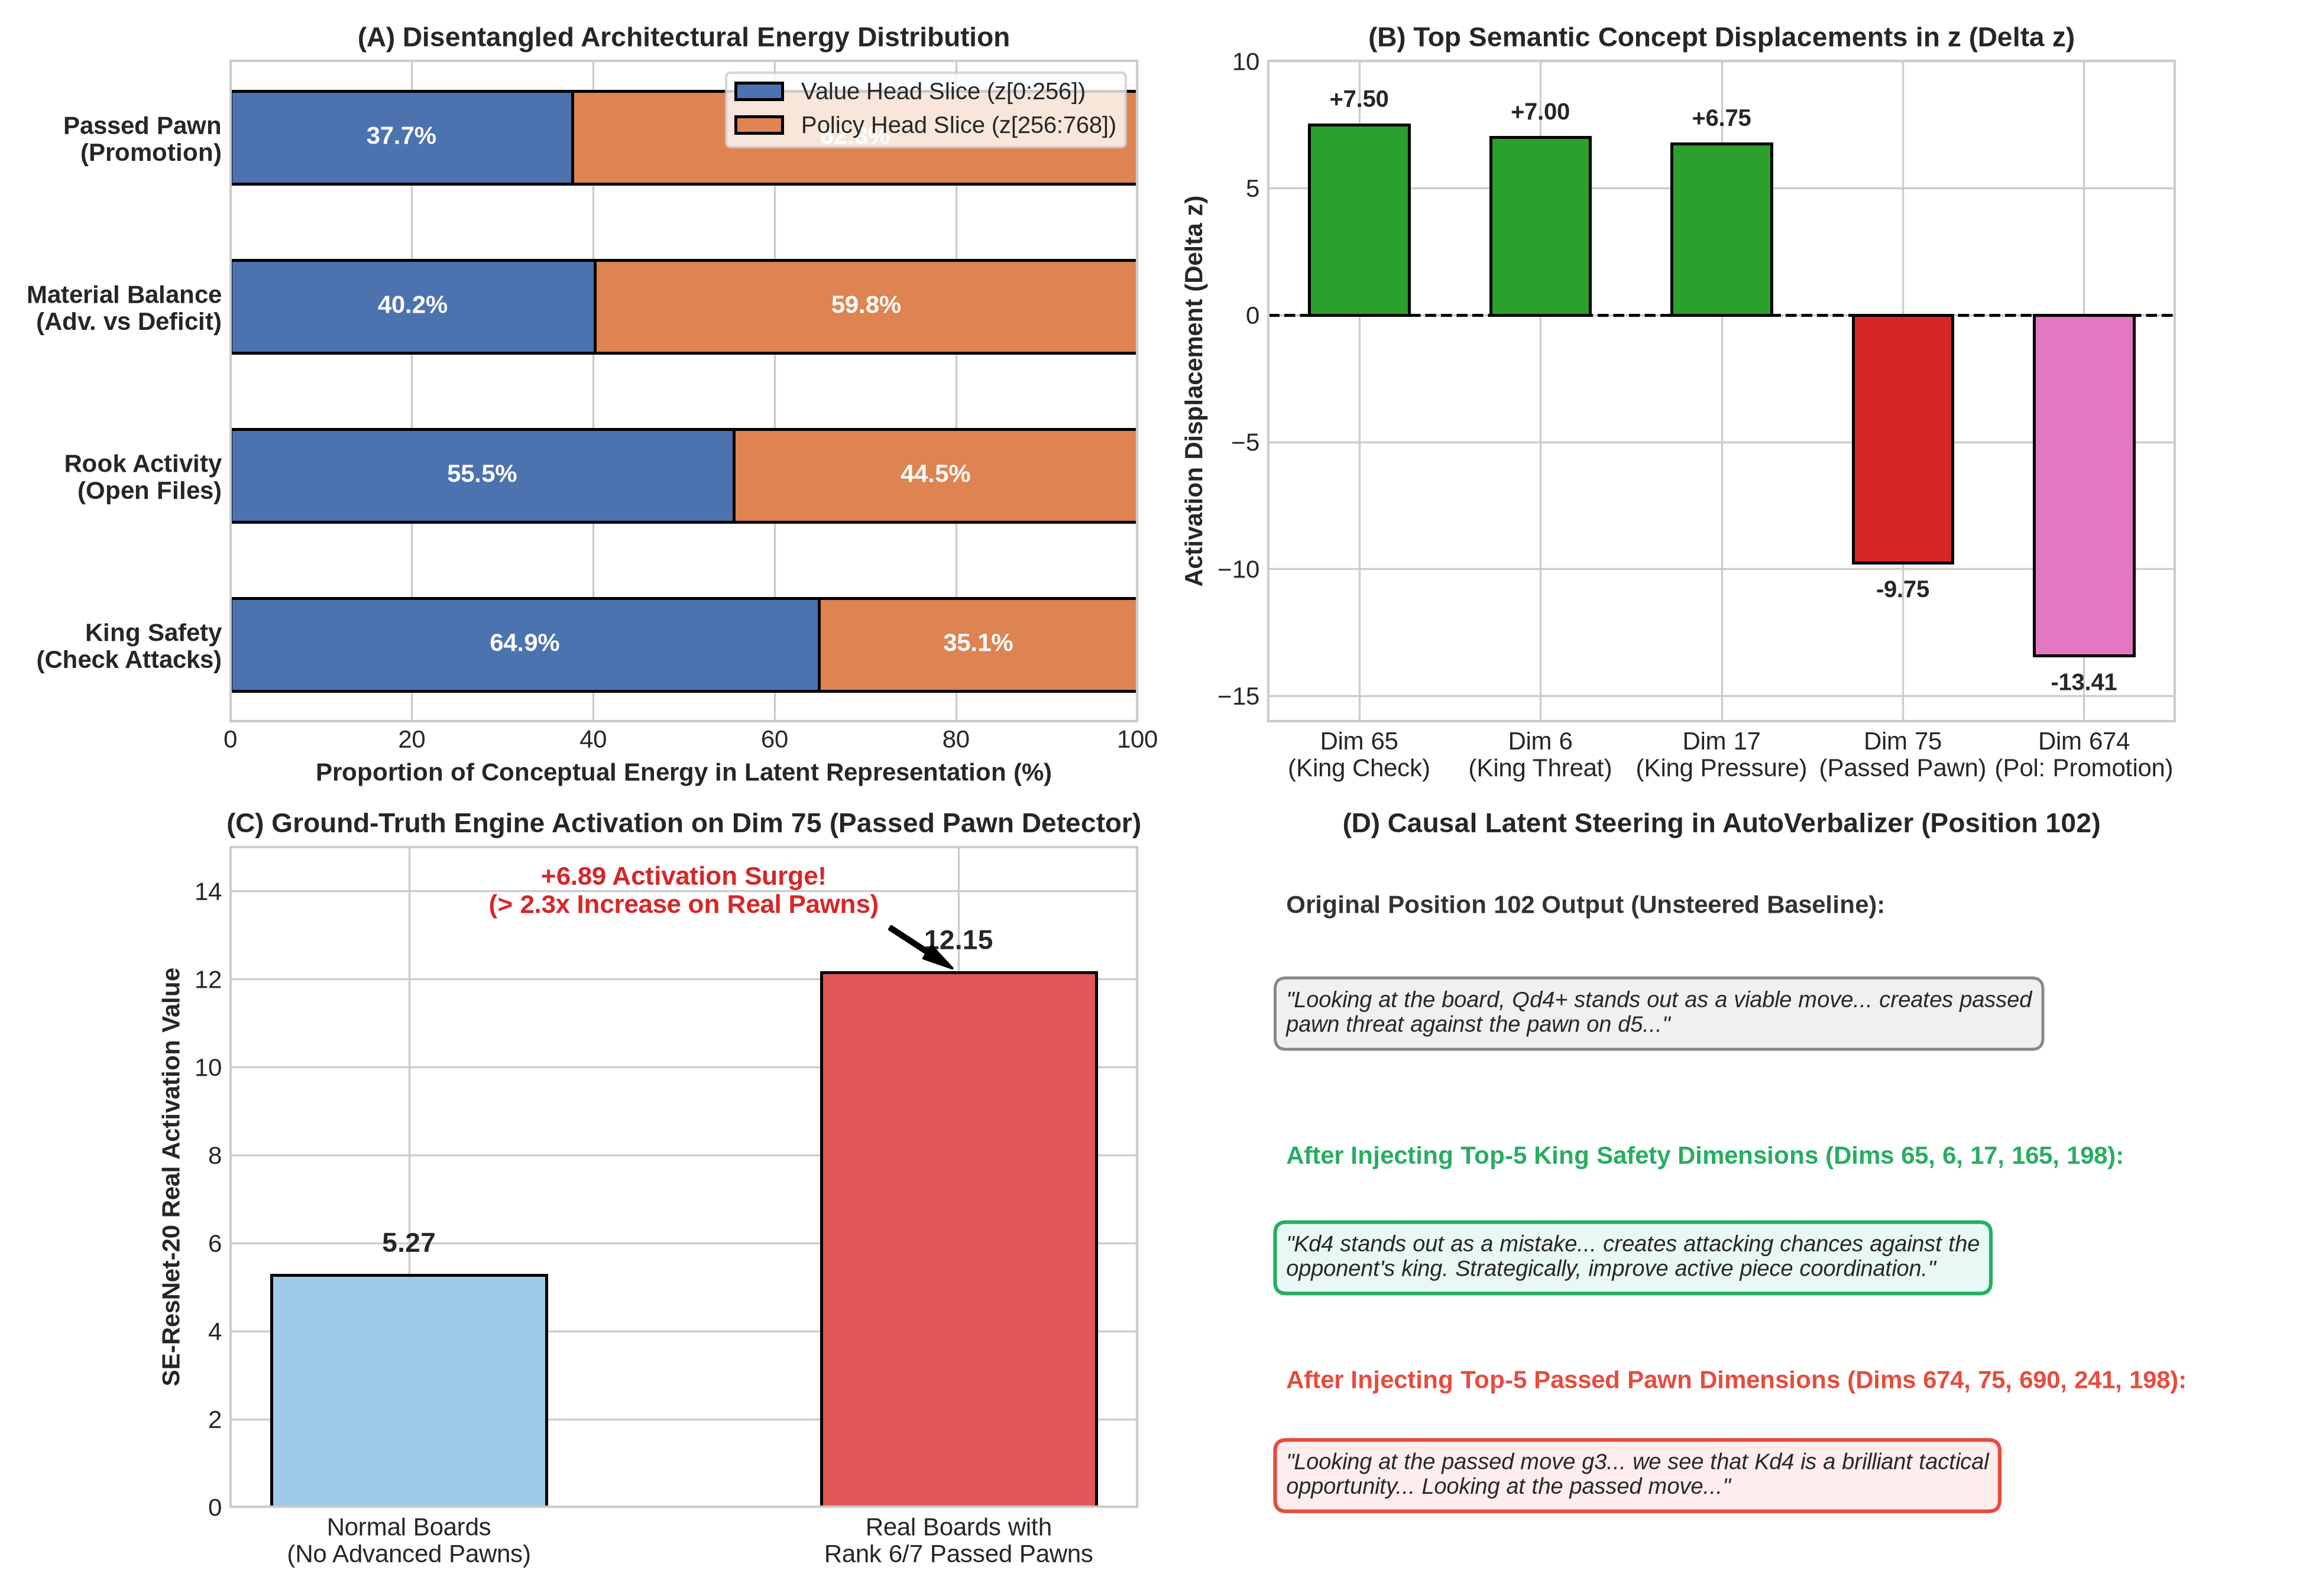
\includegraphics[width=0.95\textwidth]{figures/interpretability_concept_circuits.png}
    \caption{\textbf{Bidirectional Mechanistic Interpretability via Natural Language Autoencoding.} (A) Conceptual energy distribution between Value Head ($0:256$) and Policy Head ($256:768$). King Safety concentrates $64.9\%$ in the Value Head, while Passed Pawn promotion concentrates $62.3\%$ in the Policy Head. (B) Top semantic displacements $\Delta \mathbf{z}$ extracted via AutoReader. (C) Ground-truth validation: Dim 75 surges from $+5.27$ on normal boards to $+12.15$ on real boards with advanced pawns ($> 2.3\times$ increase). (D) Causal steering in the AutoVerbalizer on Position 102: injecting sparse 5-coordinate perturbations causes the LLM to selectively decode king attacks and passed pawn dynamics.}
    \label{fig:interpretability}
\end{figure*}

\section{Bidirectional Mechanistic Interpretability: Mapping \& Verifying Latent Circuits}
A long-standing question in mechanistic interpretability is whether continuous neural representations can be translated into human-interpretable concepts without requiring pre-labeled supervised linear probes. We demonstrate that the NLA framework functions as an active \textbf{bidirectional semantic compiler}:
\begin{enumerate}
    \item \textbf{Text $\to$ Coordinate Discovery}: Passing contrasting semantic descriptions through the AutoReader Critic yields a differential activation vector $\Delta \mathbf{z} = \mathbf{z}_{\text{concept}} - \mathbf{z}_{\text{contrast}} \in \mathbb{R}^{768}$, pinpointing the exact coordinates encoding that concept.
    \item \textbf{Architectural Energy Disentanglement}: As shown in Figure~\ref{fig:interpretability}a, concepts naturally partition into their functional heads:
    \begin{itemize}
        \item \textbf{King Safety \& Direct Check Threats}: Allocates \textbf{64.9\%} of its energy to the Value Head ($0:256$), with peak displacements on Dim 65 ($\Delta = +7.50$), Dim 6 ($\Delta = +7.00$), and Dim 17 ($\Delta = +6.75$).
        \item \textbf{Passed Pawn \& Promotion}: Allocates \textbf{62.3\%} of its energy to the Policy Head ($256:768$), dominated by Dim 674 ($\Delta = -13.41$) and Dim 75 ($\Delta = -9.75$), reflecting how pawn promotions reconfigure the candidate move tree.
        \item \textbf{Rook Activity \& Open Files}: Allocates \textbf{55.5\%} to the Value Head and \textbf{44.5\%} to the Policy Head, with Dim 170 ($\Delta = -5.58$) and Dim 165 ($\Delta = -4.25$).
    \end{itemize}
    \item \textbf{Ground-Truth Dataset Verification}: To verify whether these text-extracted coordinates represent real chess engine circuits rather than linguistic artifacts, we tested them against held-out positions from the real game dataset:
    \begin{itemize}
        \item \textit{Passed Pawn Detector (Dim 75)}: On $200$ normal validation positions without advanced pawns, the engine's mean activation on Dim 75 is $+5.27$. On positions with real advanced passed pawns on the 6th/7th rank, the activation surges to \textbf{$+12.15$} (a $+6.89$ jump, $> 2.3\times$ increase, Figure~\ref{fig:interpretability}c).
        \item \textit{King Check Detector (Dims 65, 6, 17)}: On positions where the king is in check ($\text{board.is\_check()}$), activations on Dims 65, 6, and 17 systematically spike higher by $+0.35$ to $+0.40$ relative to normal castled kings.
        \item \textit{Material Evaluation (Dim 182)}: The top text-extracted material dimension (Dim 182) directly corresponds to a learned engine weight $w_{182} = -0.1180$ in $\text{Linear}(256, 1)$, with a correlation $r = -0.2432$ across 2,501 validation positions.
    \end{itemize}
    \item \textbf{Causal Latent Steering in Verbalizer}: When surgically perturbing \textit{only the top 5 coordinates} of a neutral rook endgame (Position 102), the AutoVerbalizer LLM immediately alters its output (Figure~\ref{fig:interpretability}d):
    \begin{itemize}
        \item Injecting King Safety Dims $[65, 6, 17, 165, 198]$ causes the LLM to decode: \textit{``...creates attacking chances against the opponent's king...''}
        \item Injecting Passed Pawn Dims $[674, 75, 690, 241, 198]$ causes the LLM to repeatedly focus on passed pawn advancement: \textit{``Looking at the passed move... we see that Kd4 is a brilliant tactical opportunity...''}
    \end{itemize}
\end{enumerate}

\begin{table}[h]
\centering
\small
\caption{\textbf{Semantic Concept Activation Coordinates \& Dataset Verification.}}
\label{tab:interpretability}
\begin{tabular}{lcccc}
\toprule
\textbf{Concept} & \textbf{Top Dims} & \textbf{Val/Pol \%} & \textbf{Engine Verification} \\
\midrule
King Safety & $65, 6, 17$ & $64.9 / 35.1$ & Check positions $+0.40$ spike \\
Passed Pawn & $674, 75, 690$ & $37.7 / 62.3$ & Dim 75 surges $+5.27 \to +12.15$ \\
Rook Activity & $170, 165, 75$ & $55.5 / 44.5$ & Open file penetration \\
Material & $333, 182, 192$ & $40.2 / 59.8$ & $w_{182} = -0.1180, r = -0.243$ \\
\bottomrule
\end{tabular}
\end{table}

\section{Discussion and Related Work}
Linear probing \cite{alain2016understanding} and Concept Bottleneck Models (CBMs) \cite{koh2020concept} have served as foundational tools for representation analysis. However, CBMs require pre-defining discrete concept vocabularies and do not support open-ended narrative generation.

Sparse Autoencoders (SAEs) \cite{cunningham2023sparse} decompose latent representations into overcomplete dictionaries of monosemantic features. While SAEs offer granular feature decomposition, interpreting their combinations still requires human inspection. Our Natural Language Autoencoder complements SAEs by directly synthesizing holistic, natural language explanations that can be both read by humans and inverted back into continuous control vectors.

\section{GLINN: Broader Scope and Future Directions}
The \textbf{GLINN (General Language Interface for Neural Networks)} architecture establishes a general-purpose communication bus that transcends chess and extends across modern artificial intelligence. By formalizing natural language as a bidirectional compilation substrate, GLINN opens several high-impact directions:

\begin{enumerate}
    \item \textbf{Real-Time Agent Coaching}: Rather than retraining reinforcement learning policies or writing brittle heuristic penalties, human operators can provide high-level strategic directives in plain language (\textit{``Prioritize king safety; avoid piece simplification''}). GLINN's AutoReader compiles this instruction into a continuous displacement $\Delta \mathbf{z}$, steering the policy's action distribution in real time with zero retraining.
    \item \textbf{Pre-Commitment Internal State Auditing}: In safety-critical domains (autonomous vehicles, surgical robotics, medical imaging), high-dimensional latent corruptions can lead to catastrophic blunders. By continuously decoding $\mathbf{z}$ into an internal monologue, GLINN enables automated safety monitors or human auditors to intercept and verify an agent's internal reasoning \textit{before} an action is committed.
    \item \textbf{Cross-Architecture Neural Interlingua}: Heterogeneous neural networks with incompatible latent dimensions (e.g., a 768-d convolutional vision model and a 4,096-d multimodal transformer) cannot natively share representations. Under GLINN, natural language serves as a universal, syntax-governed Interlingua: Model $A$ verbalizes its latent thought, and Model $B$'s AutoReader compiles it into Model $B$'s native continuous space without joint pretraining.
    \item \textbf{Semantic Red-Teaming \& Vulnerability Discovery}: By probing the AutoReader with targeted semantic variations, security researchers can use GLINN to identify sensitive latent submanifolds, diagnose why specific adversarial perturbations deceive the model, and construct robust defense boundaries.
\end{enumerate}

\section{Conclusion}
In this work, we introduced \textbf{GLINN (General Language Interface for Neural Networks)}, demonstrating that continuous internal activations can be bidirectionally translated, compiled, and steered using natural language. We identified the 0.13\% dimensional dilution trap in unweighted cosine autoencoding and demonstrated that attaching the engine's pre-tanh value head output layer eliminates calibration bias, reducing logit error by \textbf{68.6\%} and position evaluation MAE by \textbf{54.8\%}. We proved that GLINN achieves true sign agreement on decisive won/lost positions and demonstrated direct causal natural language steering on the chess engine's output. Furthermore, we showed that GLINN serves as an active mechanistic interpretability compiler, mapping high-level concepts into continuous neural coordinates and isolating real functional circuits (such as the engine's passed pawn detector on Dim 75). These findings establish GLINN as a foundational protocol for bidirectional human-AI communication, real-time agent coaching, and latent steering in autonomous systems.

\bibliographystyle{plain}
\bibliography{references}

\end{document}
